\documentclass[11pt]{article}
\usepackage[margin=1in]{geometry}
\usepackage{amsmath,amssymb,amsthm}
\usepackage{booktabs}
\usepackage{graphicx}
\usepackage{float}
\usepackage{hyperref}

\newcommand{\E}{\mathbb{E}}
\newcommand{\R}{\mathbb{R}}
\DeclareMathOperator*{\argmin}{arg\,min}
\newtheorem{theorem}{Theorem}
\newtheorem{lemma}{Lemma}

\title{Data 37711 Homework 3 --- Problem 2\\
\large Hyper-parameter selection and generalization}
\author{Yiwen Chen}
\date{}

\begin{document}
\maketitle
\sloppy

The code for the simulation in (b) and the experiments in (c) is in \texttt{problem2.py}.

%==========================================================================
\section*{(a) A generalization bound for selecting hyper-parameters on a test set}

\paragraph{Setup.}
Let $D_n$ be a training set of $n$ i.i.d.\ draws from a distribution $P$ on
$\mathcal X\times\mathcal Y$. Fix a finite grid of hyper-parameter values $\theta_1,\dots,\theta_k$
\emph{before} looking at the test set. The learning algorithm maps $(D_n,\theta_j)$ to a predictor
$\hat h_j$. Let $S=\{(x_i,y_i)\}_{i=1}^l$ be a test set of $l$ i.i.d.\ draws from $P$, independent
of $D_n$. Assume the loss is bounded, $\ell(\hat y,y)\in[0,B]$. Write
\[
R(h)=\E_{(X,Y)\sim P}\,\ell\bigl(h(X),Y\bigr),\qquad
\widehat R_S(h)=\frac1l\sum_{i=1}^l\ell\bigl(h(x_i),y_i\bigr).
\]
The procedure picks $\hat\jmath=\argmin_j\widehat R_S(\hat h_j)$ and reports
$\widehat R_S(\hat h_{\hat\jmath})$ as the estimated risk.

\begin{theorem}
For every $\delta\in(0,1)$, with probability at least $1-\delta$ over $D_n$ and $S$,
\[
\bigl|\widehat R_S(\hat h_{\hat\jmath})-R(\hat h_{\hat\jmath})\bigr|
\;\le\;\max_{1\le j\le k}\bigl|\widehat R_S(\hat h_j)-R(\hat h_j)\bigr|
\;\le\;\varepsilon(k,l,\delta):=B\sqrt{\frac{\log(2k/\delta)}{2l}} .
\]
On the same event the selected model is also nearly as good as the best of the $k$ candidates:
$R(\hat h_{\hat\jmath})\le\min_jR(\hat h_j)+2\varepsilon(k,l,\delta)$.
\end{theorem}

\begin{lemma}[Hoeffding]
If $Z_1,\dots,Z_l$ are i.i.d., $Z_i\in[0,B]$ and $\E Z_i=\mu$, then for every $\varepsilon>0$,
$\Pr\bigl(\bigl|\frac1l\sum_iZ_i-\mu\bigr|>\varepsilon\bigr)\le2\exp(-2l\varepsilon^2/B^2)$.
\end{lemma}
\begin{proof}[Proof sketch]
For $s>0$, Markov's inequality applied to $e^{s\sum_i(Z_i-\mu)}$, together with independence,
gives
$\Pr(\bar Z-\mu>\varepsilon)\le e^{-sl\varepsilon}\prod_i\E e^{s(Z_i-\mu)}$.
Hoeffding's lemma says that a variable with mean zero taking values in an interval of length $B$
satisfies $\E e^{s(Z_i-\mu)}\le e^{s^2B^2/8}$. So the bound is
$\exp(-sl\varepsilon+ls^2B^2/8)$. Taking $s=4\varepsilon/B^2$ gives $e^{-2l\varepsilon^2/B^2}$.
The lower tail is the same bound applied to $-Z_i$. Adding the two tails gives the factor 2.
\end{proof}

\begin{proof}[Proof of the theorem]
\emph{Step 1 (condition on training).} Condition on $D_n$ (and on any internal randomness of the
learner, e.g.\ random-forest seeds). Then $\hat h_1,\dots,\hat h_k$ are fixed functions. Because
$S$ is independent of $D_n$, the test points are still i.i.d.\ from $P$ given $D_n$. Hence, for
each \emph{fixed} $j$, the variables $Z^{(j)}_i=\ell(\hat h_j(x_i),y_i)$, $i=1,\dots,l$, are
i.i.d., lie in $[0,B]$, and have mean $R(\hat h_j)$.

\emph{Step 2 (one model).} By Hoeffding,
$\Pr\bigl(|\widehat R_S(\hat h_j)-R(\hat h_j)|>\varepsilon\,\big|\,D_n\bigr)\le2e^{-2l\varepsilon^2/B^2}$.

\emph{Step 3 (union bound over the grid).}
\[
\Pr\Bigl(\max_j|\widehat R_S(\hat h_j)-R(\hat h_j)|>\varepsilon\,\Big|\,D_n\Bigr)
\le\sum_{j=1}^k\Pr\bigl(|\widehat R_S(\hat h_j)-R(\hat h_j)|>\varepsilon\,\big|\,D_n\bigr)
\le2k\,e^{-2l\varepsilon^2/B^2}.
\]
Setting the right-hand side to $\delta$ gives $\varepsilon=B\sqrt{\log(2k/\delta)/(2l)}$. The
bound does not depend on $D_n$, so taking the expectation over $D_n$ shows that the unconditional
probability is also at most $\delta$.

\emph{Step 4 (the selected model).} The index $\hat\jmath$ depends on $S$. So
$\widehat R_S(\hat h_{\hat\jmath})$ is \emph{not} an average of i.i.d.\ terms with mean
$R(\hat h_{\hat\jmath})$, and Step 2 cannot be applied to it directly. This is why the union bound
is needed. But $\hat\jmath\in\{1,\dots,k\}$ always, so on the event of Step 3 the deviation of
$\hat h_{\hat\jmath}$ is at most the maximum deviation, which is at most $\varepsilon$.

Finally, let $j^\star=\argmin_jR(\hat h_j)$. On the same event,
$R(\hat h_{\hat\jmath})\le\widehat R_S(\hat h_{\hat\jmath})+\varepsilon
\le\widehat R_S(\hat h_{j^\star})+\varepsilon\le R(\hat h_{j^\star})+2\varepsilon$.
\end{proof}

\paragraph{Remarks.}
\begin{itemize}
\item \textbf{Dependence on $n$, $l$, $k$.} The gap shrinks like $\sqrt{\log k/l}$. It grows only
logarithmically in the number of hyper-parameter settings and does \emph{not} depend on $n$.
The training-set size affects \emph{how good} the candidates $R(\hat h_j)$ are, not how accurately
the test set measures them. If we also want to compare with the best predictor in each model class,
a training-set bound has to be added, e.g.\ for ERM over finite classes $\mathcal H_j$,
$R(\hat h_j)\le\inf_{h\in\mathcal H_j}R(h)+2B\sqrt{\log(2k|\mathcal H_j|/\delta)/(2n)}$ for all $j$
simultaneously. That term carries the $n$-dependence.
\item \textbf{The bias of the reported number.} The same argument in expectation bounds the
optimism of the reported test risk. Each $R(\hat h_j)-\widehat R_S(\hat h_j)$ is sub-Gaussian with
variance proxy $B^2/(4l)$, and the maximal inequality for $k$ sub-Gaussians gives
\[
0\;\le\;\E\bigl[R(\hat h_{\hat\jmath})-\widehat R_S(\hat h_{\hat\jmath})\bigr]\;\le\;B\sqrt{\frac{\log k}{2l}} ,
\]
and the lower bound $0$ always holds (see (b)). So the reported number is optimistic on average, by
at most order $B\sqrt{\log k/l}$.
\item \textbf{Tightness.} The $\sqrt{\log k/l}$ rate cannot be improved in general. The example
in (b) attains it.
\end{itemize}

%==========================================================================
\section*{(b) Using the same test set for selection and for evaluation}

\paragraph{1. The reported risk is biased downwards.}
For each fixed $j$, $\widehat R_S(\hat h_j)$ is an unbiased estimate of $R(\hat h_j)$. But we report
the \emph{minimum} of $k$ noisy estimates, so
\[
\E\bigl[\widehat R_S(\hat h_{\hat\jmath})\bigr]=\E\bigl[\min_j\widehat R_S(\hat h_j)\bigr]
\le\min_j\E\bigl[\widehat R_S(\hat h_j)\bigr]=\min_jR(\hat h_j)\le\E\bigl[R(\hat h_{\hat\jmath})\bigr]
\]
(conditionally on $D_n$). The inequality is strict as soon as several candidates are close. This is
a ``winner's curse''. The model that wins is partly the best model and partly the luckiest one on
this particular test set. Any confidence interval computed as if one fixed model had been evaluated
(width $\propto1/\sqrt l$) is too narrow, because it ignores the $\sqrt{\log k}$ factor.

\paragraph{2. When $k$ is large relative to $l$ the test set is overfit.}
The bound in (a) is informative only when $\log k\ll l$. Once $\log k$ is comparable to $l$ it is
vacuous, and this is not just looseness. Consider $k$ classifiers that each guess labels at random,
so that every one has true error exactly $1/2$. Each test error is $\mathrm{Bin}(l,1/2)/l$, and the
smallest of $k$ such values is about $\tfrac12-\sqrt{\log k/(2l)}$, which is the rate in (a).
\begin{itemize}
\item With $l=100$, the simulation in Figure~\ref{fig:sim} gives a reported error of
$\mathbf{0.339}$ for $k=1000$ and $\mathbf{0.285}$ for $k=10^5$, although no model is better
than a coin flip.
\item If $k\ge2^l$, the grid can contain a predictor that labels \emph{every} test point correctly.
The reported test error is then $0$ while the true error is $1/2$.
\end{itemize}
In effect the selection step becomes a learning algorithm whose training set is the test set. With
$k$ choices it can memorize about $\log_2k$ bits of the test labels. A large grid, or a continuous
hyper-parameter searched finely (learning rate, random seed, early-stopping epoch, \dots), quickly
reaches that regime when $l$ is small.

\paragraph{3. Further problems.}
(i) The \emph{choice itself} becomes noisy. When many settings have similar true risk, the winner
is decided largely by test-set noise. The oracle inequality still guarantees
$R(\hat h_{\hat\jmath})\le\min_jR(\hat h_j)+2\varepsilon$, but $\varepsilon$ is large when $k$ is
large relative to $l$. (ii) In practice the grid is often \emph{adapted} after looking at test
scores (refine around the best value, try another model, \dots). Then the candidates are not fixed
in advance and the union bound over $k$ fixed models no longer applies. The effective number of
models can be much larger than the number actually fit (adaptive overfitting, the ``leaderboard''
problem).

\paragraph{Remedy.} Use one data set to \emph{select} (a validation set, or cross-validation on the
training data) and a separate, untouched test set to \emph{evaluate} the single selected model once.
On the test set the selected model is then a fixed function, so (a) applies with $k=1$:
$|\widehat R_{\text{test}}-R|\le B\sqrt{\log(2/\delta)/(2l_{\text{test}})}$, and the estimate is
unbiased. Part (c) does exactly this.

\begin{figure}[H]\centering
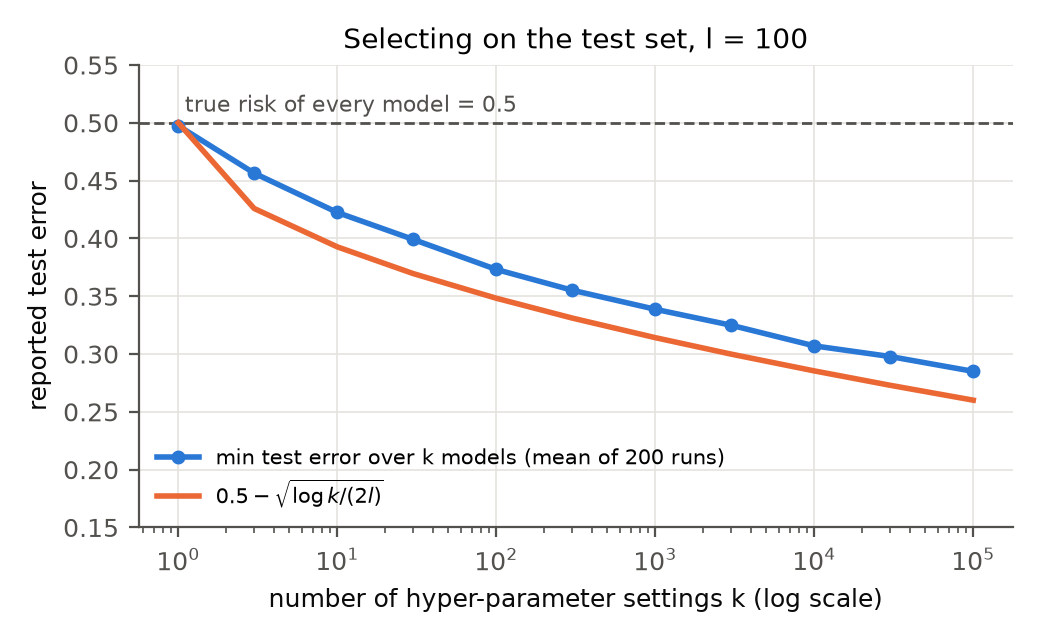
\includegraphics[width=0.62\textwidth]{problem2_selection_simulation.png}
\caption{Selecting the best of $k$ useless classifiers (true error $0.5$) on a test set of $l=100$
points. The blue curve is the minimum test error, averaged over 200 repetitions. The orange curve is
the $\tfrac12-\sqrt{\log k/(2l)}$ rate from the union bound.}
\label{fig:sim}
\end{figure}

%==========================================================================
\section*{(c) Train / validation / test on the white-wine data}

\paragraph{Data and split.} \texttt{winequality-white.csv} has 4898 wines, 11 physico-chemical
covariates, and the target \texttt{quality}, which takes values $3$--$9$ in this file. The file is
split at random (seed 0) into \textbf{3428 train (70\%), 490 validation (10\%) and 980 test (20\%)}
points. The loss is MSE. For reference, predicting the training mean ($5.90$) gives validation MSE
$0.784$ and test MSE $0.888$.

\paragraph{Model classes and hyper-parameters.} I chose \texttt{RandomForestRegressor} and
\texttt{KNeighborsRegressor}. Each grid has \textbf{600 settings, more than the 490 validation
points}, as required.
\begin{itemize}
\item \textbf{Random forest}, $3\times4\times5\times5\times2=600$ settings.
\texttt{n\_estimators}$\in\{50,150,300\}$ is the number of trees. More trees reduce the variance of
the average and do not cause overfitting. \texttt{max\_depth}$\in\{\text{None},5,10,20\}$ and
\texttt{min\_samples\_leaf}$\in\{1,2,4,8,16\}$ control how complex each tree is: shallow trees or
large leaves mean more bias and less variance. \texttt{max\_features}$\in\{0.1,0.3,0.5,0.7,1.0\}$ is
the fraction of the 11 features tried at each split. Smaller values decorrelate the trees, and $1.0$
is plain bagging. \texttt{bootstrap}$\in\{\text{True},\text{False}\}$ says whether each tree sees a
bootstrap resample or the full training set.
\item \textbf{$k$-nearest neighbours}, $2\times50\times2\times3=600$ settings.
\texttt{n\_neighbors}$\,=k\in\{1,\dots,50\}$ is the main bias--variance knob: small $k$ is wiggly,
large $k$ is smooth. \texttt{weights}$\in\{$uniform, distance$\}$ chooses between a plain average
and an inverse-distance-weighted average of the neighbours. The distance is
\texttt{metric}$\in\{$manhattan, euclidean, chebyshev$\}$. Because KNN depends on the scale of the
features, the preprocessing (\texttt{StandardScaler} or \texttt{MinMaxScaler}, fit on the training
set) is treated as a hyper-parameter too.
\end{itemize}
Every setting is fit on the training set and scored on the validation set. The setting with the
smallest validation MSE is selected, and its test MSE is reported. The script also stores the test
MSE of \emph{every} setting, but only to study the validation--test relationship afterwards. It is
never used for selection.

\begin{table}[H]\centering\small\setlength{\tabcolsep}{4pt}
\begin{tabular}{lcc}
\toprule
 & random forest & KNN\\
\midrule
selected setting & \begin{tabular}[t]{@{}c@{}}150 trees, max\_depth 20,\\ min\_samples\_leaf 1,\\ max\_features 0.1, no bootstrap\end{tabular}
 & \begin{tabular}[t]{@{}c@{}}standard scaling,\\ $k=12$, distance weights,\\ Manhattan distance\end{tabular}\\
\midrule
train MSE & 0.003 & 0.000\\
validation MSE (selected) & \textbf{0.363} & \textbf{0.381}\\
\textbf{test MSE (selected)} & \textbf{0.461} & \textbf{0.496}\\
test $R^2$ (vs.\ mean baseline) & 0.48 & 0.44\\
\midrule
best test MSE in grid (oracle) & 0.455 & 0.483\\
test-MSE rank of the selected setting (of 600) & 8 & 14\\
val.--test corr.\ (Pearson / Spearman) & 0.97 / 0.99 & 0.95 / 0.94\\
test $-$ val.\ MSE, selected setting & 0.097 & 0.115\\
test $-$ val.\ MSE, mean over 600 settings & 0.102 & 0.112\\
\bottomrule
\end{tabular}
\caption{Grid-search results on the main split (seed 0).}
\label{tab:wine}
\end{table}

\paragraph{Test performance.} The selected random forest has \textbf{test MSE $0.461$} and the
selected KNN has \textbf{test MSE $0.496$}. Both roughly halve the error of the mean predictor
($0.888$), and the random forest is better. Both winners are low-bias, ``memorizing'' settings: a
fully grown, un-bootstrapped forest with one random feature per split, and distance-weighted KNN.
Both have training MSE $\approx0$. Part of the reason is that the file contains \textbf{937 exact
duplicate rows}. $28.6\%$ of the validation rows and $24.5\%$ of the test rows have an exact copy
(including the label) in the training set, and memorizing models predict those copies perfectly.
This affects validation and test in the same way, so the model comparison is fair. But the
absolute MSEs are somewhat optimistic for genuinely new wines.

\begin{figure}[H]\centering
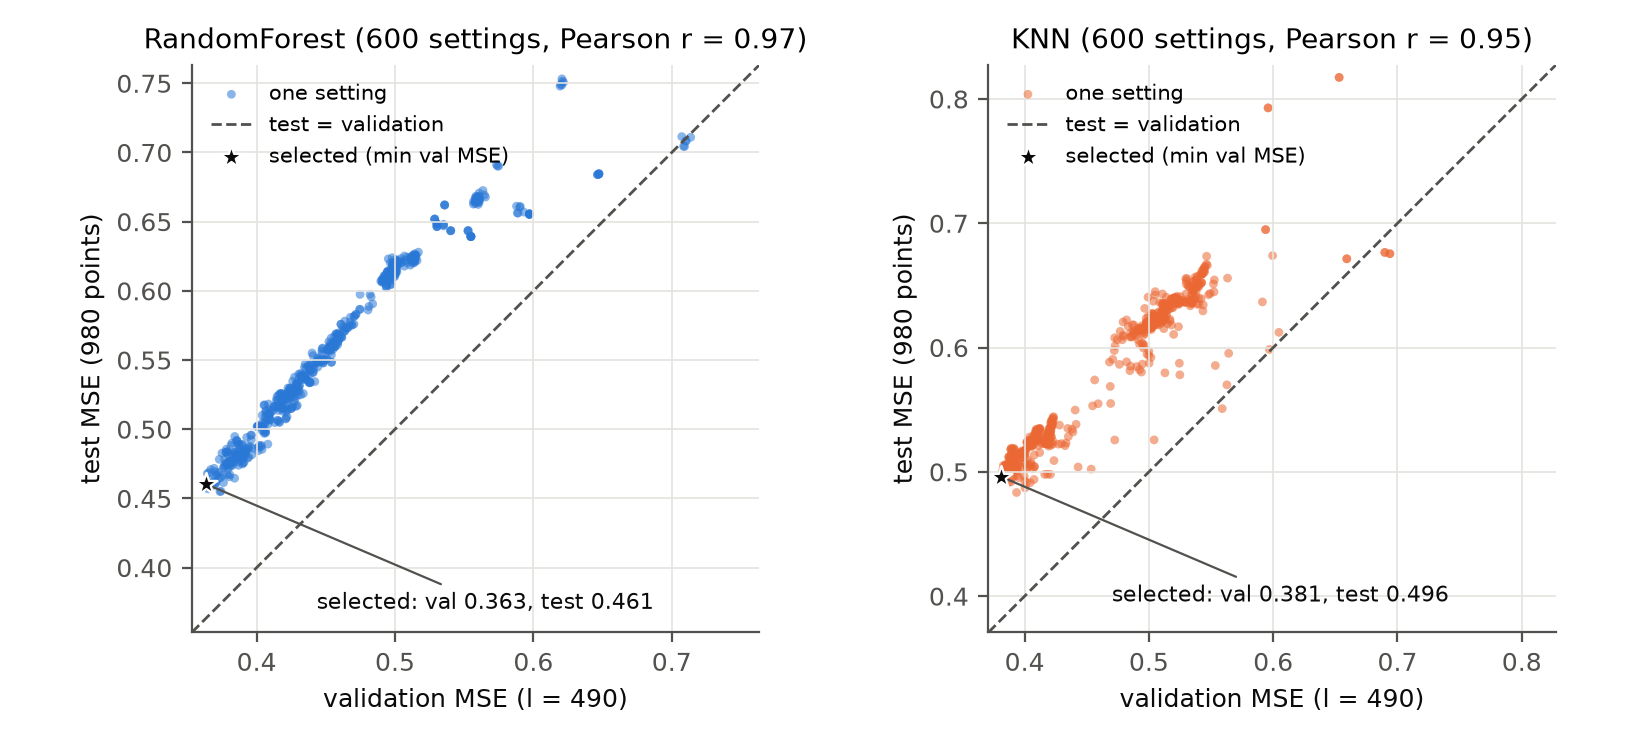
\includegraphics[width=\textwidth]{problem2_val_vs_test.png}
\caption{Validation MSE (490 points) vs.\ test MSE (980 points) of all 600 settings of each model
class. The star is the setting selected by validation MSE.}
\label{fig:valtest}
\end{figure}

\begin{figure}[H]\centering
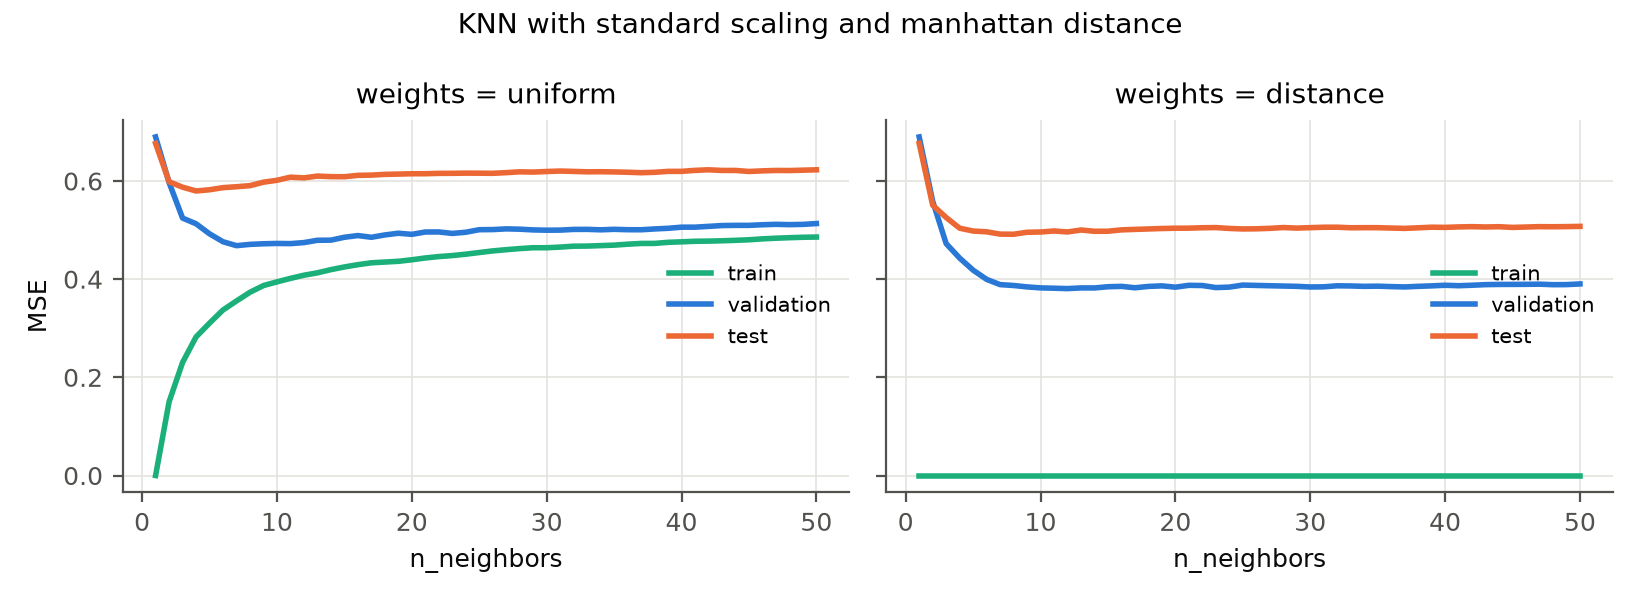
\includegraphics[width=\textwidth]{problem2_knn_curves.png}
\caption{KNN train / validation / test MSE as a function of $k$, for the selected scaling and
metric. The validation curve tracks the shape of the test curve, shifted down by about $0.1$ on this
split.}
\label{fig:knn}
\end{figure}

\paragraph{Relationship between validation risk and test risk.}
\begin{enumerate}
\item \textbf{The validation set ranks the models well.} Across the 600 settings, validation and
test MSE are almost perfectly monotonically related (Spearman $0.99$ for RF and $0.94$ for KNN,
Figure~\ref{fig:valtest}). The selected setting is the 8th (RF) and 14th (KNN) best of 600 on the
test set, only $0.006$ and $0.013$ worse than the best test MSE in the grid. This is the oracle
inequality of (a) at work: selecting on held-out data finds a nearly optimal setting.

\item \textbf{The selected validation MSE underestimates the test MSE.} On this split the gap is
large ($0.097$ for RF, $0.115$ for KNN), but it is \emph{not} mainly caused by the selection. The
gap is almost the same for \emph{every} setting (on average $0.102$ and $0.112$), i.e.\ all points
in Figure~\ref{fig:valtest} lie above the diagonal by about the same amount. This particular
validation sample is simply easier than the test sample: its label variance is $0.78$ vs.\ $0.88$,
and it has more training duplicates ($28.6\%$ vs.\ $24.5\%$). With $l=490$, the standard error of a
single validation MSE is about $0.04$, so a shift of $0.1$ is about two standard errors of ordinary
sampling noise. The part of the gap due to selection is the selected gap minus the average gap,
$-0.005$ (RF) and $+0.004$ (KNN), which is negligible on this split.

\item \textbf{On average, the selection makes the validation score optimistic.} To separate
selection bias from the luck of one split, I repeated the whole KNN grid search on 20 further random
70/10/20 splits (\texttt{problem2\_knn\_repeated\_splits.csv}). The selected setting had mean
validation MSE $0.378$ and mean test MSE $0.405$. That is an \textbf{optimism of $0.027\pm0.009$}
(s.e.), and test exceeded validation in 14 of the 20 splits. For a single \emph{fixed} model the
validation MSE is unbiased, so this systematic gap is exactly the winner's curse of (b):
$\E[\min_j\widehat R_{\text{val}}(\hat h_j)]\le\min_jR(\hat h_j)$. The selected model's test MSE
was on average only $0.009$ above the best test MSE in the grid, so the \emph{choice} was good even
though the \emph{score} of the choice was optimistic.

\item \textbf{Comparison with the bound in (a).} The predictions of both models are averages of
training labels, so $\hat y,y\in[3,9]$ and the squared loss lies in $[0,B]$ with $B=36$. With
$k=600$, $l=490$ and $\delta=0.05$, the bound gives $\varepsilon=36\sqrt{\log(24000)/980}=3.65$,
which is vacuous next to MSEs of about $0.4$. The observed optimism ($0.027$) is much smaller, for
two reasons. (i) Hoeffding uses the worst-case range $B=36$, while the squared errors are usually
far below $1$; a variance-sensitive (Bernstein-type) bound would be much tighter. (ii) The 600
settings are highly correlated, since neighbouring values of $k$ give nearly the same predictions,
so the effective number of distinct models is much smaller than $600$. Even for independent models,
a $\sqrt{2\log600}\approx3.6$ multiple of the $0.04$ standard error would be about $0.14$.
Correlation brings it down to the observed $\approx0.03$.
\end{enumerate}

\paragraph{Conclusion.} The validation risk of the selected model is a slightly optimistic
estimate of its true risk, and on any single split it also carries the sampling noise of only 490
points. The test set, which was not used for any decision, gives the honest estimate:
\textbf{random forest $0.461$, KNN $0.496$}. The selected models are also nearly the best the grids
contain, so with $l=490$ and $\log k\approx6.4$ the validation set was large enough for selection to
work, even though it could not certify the final error by itself.

\end{document}
